\firstsection{Introduction}

\maketitle

Convolutional neural networks (CNNs) have been successfully applied to a wide range of visual tasks, most famously to natural image object recognition~\cite{krizhevsky_imagenet2012, simonyan_very_deep2014, szegedy2015}, for which some claim equivalent or better than human performance. This performance comparison is often motivated by the idea that CNNs model or reproduce the early layers of the visual cortex, even though they do not incorporate many details of biological neural networks or model higher-level abstract or symbolic reasoning~\cite{yamins2016using, hassabis2017neuroscience, human_vs_machine_vision}. While CNN techniques were originally inspired by neuroscientific discoveries, recent advances in processing larger datasets with deeper networks have been the direct results of engineering efforts. Throughout this significant advancement, researchers have aimed to understand why and how CNNs produce such high performance~\cite{goodfellow_book, deeplearning_blackbox2017}, with recent works targeting the systematic evaluation of the visual perception limits of CNNs~\cite{clevr, not_so_clevr}.

One fundamental application of human vision is to understand data visualizations. This is a task unlike natural image processing but includes the abstraction of real-world objects and their effects into data, represented with visual marks. As a field, visualization catalogues and evaluates human perception of these marks, such as in the seminal \emph{graphical perception} experiments of Cleveland and McGill~\cite{cleveland_mcgill}. This work describes nine elementary perceptual reasoning tasks, such as position relative to a scale, length, angle, area, and shading density, plus orders their reasoning difficulty. But, with increasing research interest in the machine analysis of graphs, charts, and visual encodings, it seems pertinent to question whether CNNs are able to process these basic graphical elements and derive useful measurements from the building blocks of information visualization.

As such, we reproduce Cleveland and McGill's human perceptual experiments with CNNs, and discuss to what extent they have `graphical perception'. To perform this evaluation, we parametrize the elementary perceptual tasks and experiments suggested by Cleveland and McGill~\cite{cleveland_mcgill}, and define a set of regression tasks to estimate continuous variables. Against human perception, we pit four neural networks: a three-layer multilayer perceptron (MLP), the LeNet 2-layer CNN~\cite{lenet}, the VGG 16-layer CNN~\cite{simonyan_very_deep2014}, and the Xception 36-layer CNN~\cite{xception}. As CNNs trained on natural images are said to mimic layers of the human visual cortex, we investigate whether using weights trained on natural images (via ImageNet~\cite{imagenet}) or weights trained from scratch on elementary graphical perception tasks produces more accurate measurements and greater generalization.

We test these four networks across four scenarios presented by Cleveland and McGill~\cite{cleveland_mcgill}: 1) Nine elementary perceptual tasks with increasing parameteric complexity, e.g., length estimation with fixed x, then with varying x, then with varying width, including cross-network evaluations testing the generalizability of networks to unseen parameters; 2) The position-angle experiment, which compares judgements of bar charts to pie charts, 3) The position-length experiment, which compares grouped and divided bar charts, and 4) The bars and framed rectangles experiments, where visual cues aid ratio perception. We also investigate whether our CNNs can detect a proportional change in a measurement across scales, in relation to Weber's law.

With these experiments, we describe a ranking defining the ease with which our tested CNN architectures can estimate elementary perceptual tasks, as an equivalent to Cleveland and McGill's ranking for human perception. Further, we discuss the implications of our results and derive recommendations for the use of CNNs in perceiving visualizations. We accompany this paper with open source code and our input and results data, both to enable reproduction studies and to spur new machine perception systems more adept at graphical perception: \url{http://rhoana.org/perception}


%Cleveland and McGill's work in the 1980s has led to many insights for modern information visualization research such as the identification of elementary perceptional tasks or that bar charts are easier to understand than pie charts. 


%\emph{Can we leverage decades of visualization research to understand the way convolutional neural networks process data?}
%
%Information visualization has been an established research field for decades which has resulted in numerous insightful findings in regards to how human beings can best process information visually.
%Unpublished preliminary experiments have shown that data representations customized for the human eye also can improve the performance of an automatic classifier. 
%While the reasons for this are still unknown, specified research can most certainly advance the understanding of deep neural networks.
%
%\subsection{From Biological Vision to Machine Learning}
%
%%\begin{figure}[t]
%%	  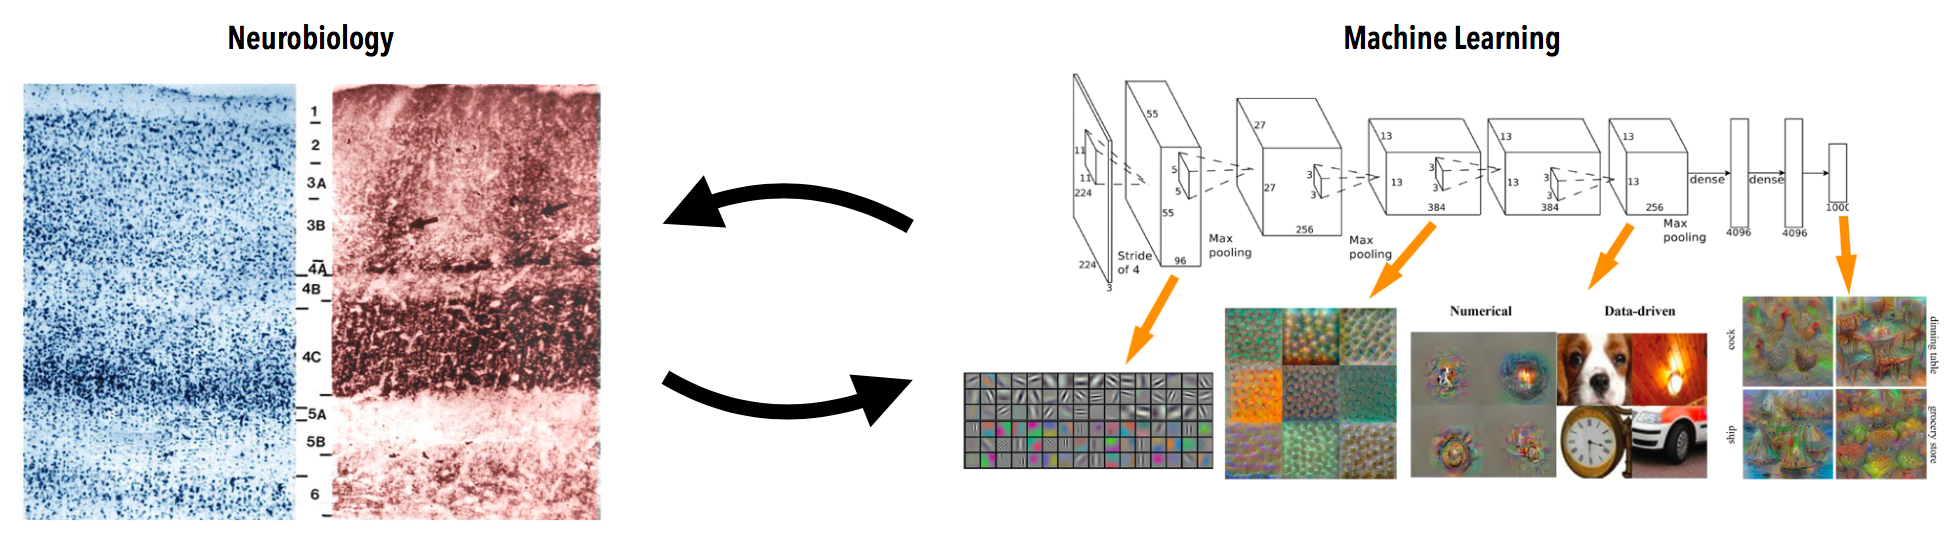
\includegraphics[width=\linewidth]{biology_vs_cnn.png}
%%  \caption{The Biological Vision (schematic)}
%%	\label{fig:vision}
%%\end{figure}
%
%Biological vision is an extremely powerful system which allows humans the ability, and seemingly without effort, to recognize an enormous amount of distinct objects in the world. 
%Object detection is extremely difficult and therefore is especially impressive as light intensities can change by levels of magnitude and contrast between foreground and background is so often low. 
%In addition, the visual scene changes every time the human body or human eyes move. 
%This visual system exhibits a very noisy structure but because it is organized by layers it has inspired the mathematical theory of multilayer neural networks. 
%What is remarkable is that even though current machine learning models do not resemble the complexity of its biological pendant, they inherently generalize extremely well. 
%Neural networks trained on one specific task can be used to perform detection or segmentation of, seemingly, unrelated objects with relatively minor retraining. 
%The reported classification performance is superior to that of humans and the question in regards to their functionality opens an interesting research topic.
%
%In 1962 Hubel and Wiesel were the first to begin studying the visual cortex from the standpoint of a neuroscientist. Their experimental findings on cats and macaque monkeys suggested a hierarchy of cells with increasing complexity which was then later transferred to the hierarchical model of different layers. Twenty years later, this insight was translated to the Neocognitron quantitative model, by Fukushima and Miyake, which ultimately led to the important work of Hinton, Bengio, and LeCun in the 1980s. Their work on stochastic gradient descent approximation, and the availability of faster computer hardware then led to today’s breakthrough of deep learning networks. In the last decade, this field has exhibited rapid growth, constant evolution, and new applications in various domains.
%
%We think that the biological inspiration of modern convolutional neural networks yields the evaluation of principles of human perception with computers.
%

